% Template for ICIP-2017 paper; to be used with:
%          spconf.sty  - ICASSP/ICIP LaTeX style file, and
%          IEEEbib.bst - IEEE bibliography style file.
% --------------------------------------------------------------------------
\documentclass{article}
\usepackage{spconf,amsmath,graphicx}
\usepackage{subcaption}
\usepackage{hyperref}

\usepackage{pgfplotstable}
\usepackage{pgfplots}

\captionsetup[figure]{font=small,skip=0pt}


% Example definitions.
% --------------------
\def\x{{\mathbf x}}
\def\L{{\cal L}}

% Title.
% ------\title{Ambiguity Index for Stereo Reconstruction Based on Dynamic Programming}
\title{Stereo Ambiguity Index for Semi-Global Matching}
%
% Single address.
% ---------------
\twoauthors{Mathias Paget, Jean-Philippe Tarel}
{Universit\' e Paris-Est, COSYS, LEPSIS, IFSTTAR,\\F-77447 Marne-la-Vall\'ee, France}
{Pascal Monasse}
{LIGM (UMR 8049), \'Ecole des Ponts, UPE,\\Champs-sur-Marne, France}

\begin{document}
\ninept
%
\maketitle
%

\begin{abstract}
Stereoscopic reconstruction is important to automatic vision systems. As an intermediate step, estimating this reconstruction is not enough for good performance of the whole system, and its uncertainty must be characterized. Several methods propose uncertainty indexes based on specific data features, thus incomplete, while others are based on learning. We propose a simple index, named ambiguity index, taking into account both data and regularization, and derived directly from the optimization process. Exploiting properties of the dynamic programming, this index is an approximation of the posterior variance when Semi-Global Matching (SGM) algorithm is used for stereo reconstruction. Improvements in refining stereo reconstruction are shown on the KITTI datasets when the index is used.
\end{abstract}
\begin{keywords}
Stereo reconstruction, Discrete optimization, Dynamic Programming, Semi-Global Matching, Uncertainty index
\end{keywords}

\section{Introduction}
\label{sec:intro}

A robust and accurate perception of the environment is required for advanced driver assistance and automatic driving systems to perform driving tasks. When only cameras are used for perception, many driving tasks, where the system extracts high-level information from low-level image information, are known to challenge computer vision systems. To face these difficult and complex problems, tasks are usually decomposed into a chain of sub-problems, each sub-problem being handled by an image or computer vision process. In such an approach, the output of each process is the input of another one. Often, each process consists in the minimization of an energy. The advantage of the decomposition into sub-problems is that the propagated information is reduced along the chain; however the risk is to reduce too drastically the propagated information and to lead to inconsistent results. To solve this issue it is necessary to propagate uncertainty information in addition to the estimation result to allow the next process to integrate it in its processing. We focus here on stereoscopic reconstruction of road scenes.

When the input noise is Gaussian and the problem linear and well-posed, the uncertainty of the output is a Gaussian function characterized by the covariance matrix of the output. This covariance matrix can be formally derived from the minimized energy. When the input noise is not Gaussian, or when the problem is non-linear, the uncertainty of the output can only be approximated by a Gaussian function, but derived covariance matrix may be voluminous. Thus, only problems with a reduced number of parameters, such as for instance camera calibration, can be handled, but not stereo reconstruction, where the number of parameters is usually over one million. Rather than estimating the covariance matrix of the output, it was thus proposed to estimate an uncertainty index based on the data features which are known to harden resolution of the problem, such as texture-less regions, repetitive patterns~\cite{hu12}. The difficulty of this approach is that it is hard to fully understand the data's effect on the estimated solution due to the usual regularization term used during stereo reconstruction minimization.

This is why it was recently proposed to learn confidence on the solution from feature on data, data cost and disparity map estimate~\cite{haeusler13, spyropoulos14, park15, seki16}. Confidence has to be understood as a prediction of an error on matching over a given threshold. It is learned from data, data cost and estimated disparity map features~\cite{spyropoulos14, park15, seki16} and additionally from final energy cost~\cite{haeusler13}. Theses approaches require supervised learning and a large ground-truth database, so we aim to propose an uncertainty index using only sub-products of the optimization process itself.

Instead of trying to learn it, we investigate the possibility of building the index from the energy and the optimization process only. It appears that optimization methods based on dynamic programming, such as the discrete optimization method Semi-Global Matching (SGM)~\cite{hirschmuller08}, have very interesting properties, which allows us to estimate easily an index on the solution. This so called ambiguity index comes from intermediate costs computed during the optimization and needs a reduced amount of computation to be obtained. The proposed ambiguity index is evaluated in several experiments, showing its interest. In particular, we use it to refine the stereo reconstruction and show its ability to improve results.

\section{Stereo Reconstruction}
\label{sec:index}

The used stereo reconstruction algorithm is a simplified version of a recent method~\cite{zbontar16}, with input images assumed already in rectified geometry. Following~\cite{scharstein02}, we describe the algorithm split into four steps: matching cost computation and cost aggregation in Sec.~\ref{ss:cost}, optimization in Sec.~\ref{ss:sgm} and refinement in Sec.~\ref{ss:lr_cons}.

\subsection{Matching Cost and Aggregation}

\label{ss:cost}

In the rectified geometry, object depth is easily parameterized by the horizontal difference in position between its left and right projections, the so-called disparity. Stereo reconstruction problem is usually set as the minimization, with respect to the disparity image, of an energy which is a function of the left and right images. The Bayesian approach provides ways to derive this energy from a statistical model of the stereo reconstruction problem. The classic form of the energy is
\begin{equation}
E(D) = \sum_{p \in P}{\text{Data}(p,d_p)} + \sum_{(p,q) \in N}{\text{Prior}(d_p,d_q)},
\label{eq:global_en}
\end{equation}
where $D=(d_p)_p$ is the disparity image with $d_p$ the disparity of the pixel~$p$, $P$~is the pixel set, $N$~the set of neighbor pairs of pixels. The data term $Data$ describes how data agrees with the solution and the prior term $Prior$, used as a regularizer, encodes the wanted properties of the solution. In our case, $Data$ is set to the census dissimilarity~\cite{zabih94} between left and right pixel patches. The census is computed on a $5\times5$ pixel window and the advantage is its invariance to an increasing function on the intensities, so it can handle photometric calibration differences between the two images and partially perturbations due to aspect differences depending on the view angle. Like in~\cite{zhang09}, cross-based aggregation is performed on the data cost. By smoothing the data cost in regions of homogeneous intensities, the noise is reduced in the data cost.

The term $Prior$ is set to a function of the disparity difference, assuming that two neighbor pixels have frequently the same depth (also called fronto-parallel prior). The assumptions on the data term is not quite valid due to occlusion, reflections and specularities, as well as on the prior term due to non-frontal surfaces such as road and lateral buildings. Intents to perform more accurate modeling, for instance to handle occlusion~\cite{kolmogorov01,kolmogorovIPOL} or regularization with higher order prior~\cite{ranftl12}, lead to more difficult to optimize energies. For this reason, simple energies are often preferred and erroneous pixels of the solution are post-processed. In practice, $Prior$ is set to:
\begin{equation}
\begin{split}
\text{Prior}(i,j) = 0 & \; \; if \; i=j, \\
\text{Prior}(i,j) = P1 & \; \; if \; |i-j| = 1, \\
\text{Prior}(i,j) = P2 & \; \; otherwise,
\end{split}
\end{equation}
where $0\leq P1\leq P2$ are fixed parameters.
It thus behaves close to a $Pott$ regularization function, yet is more permissive for slow disparity variations. This allows better handling of road scenes where non-frontal planes are numerous.

\subsection{Semi-Global Matching Optimization}
\label{ss:sgm}

The energy~\eqref{eq:global_en} is a 2D first order Markov Random Field (MRF). Global optimization of such an energy is difficult, so approximate optimization algorithms have been proposed. In Semi-Global Matching (SGM) introduced by Hirschm\"uller~\cite{hirschmuller08}, the original energy is decomposed in many 1D energies whose each global optimum can be found. SGM thus consists in minimizing along ``arms'' around each considered pixel by Dynamic Programming (DP). For each pixel and vector direction $v$, a 1D energy $C_v$ is computed using the following recursion rule:
\begin{equation}
\begin{split}
C_v(p,d) = & \text{Data}(p,d) + \\
& \min_{d'}{ C_v(p-v,d') + \text{Prior}(d,d')}.
\end{split}
\end{equation}
The original $SGM$ is performed along $R=16$ directions~$v$. We consider only $R=4$ directions as in~\cite{zbontar16}, since fostering horizontal and vertical directions in the optimization achieves better results for vertical and horizontal scene objects. The energies $C_v$ are added at the current pixel and the estimate is selected at the minimal value of this energy over disparities:
\begin{equation}
\begin{split}
SGM(p,d) & = \sum_{v} C_v(p,d) - (R-1)\text{Data}(p,d) \\
d_p & = \arg\min_{d}{SGM(p,d)}.
\end{split}
\end{equation}
Because of the 1D decomposition, each pixel solution is obtained independently and thus the smoothness of the solution is not guaranteed, despite the regularization term, leading to artifacts. Smoothing the data cost with cross based aggregation reduces these artifacts.

\subsection{Left-Right Consistency (LRC) refinement}
\label{ss:lr_cons}

Since the model is not always valid, in particular at occlusions, an additional prior is introduced during post-processing, the so-called Left-Right Consistency (LRC) on disparities~\cite{mei11}. The idea is to check that for the same object point, the disparity in the left and right images are opposites. LRC check consists in comparing the disparity, of a given pixel, to the disparity at corresponding position in the other image. Three pixel categories are thus defined:
\begin{equation}
\begin{split}
\text{correct}: & \; |D_l(p) + D_r(p- d)| \leq 1 \\
\text{mismatch}: & \; |d + D_r(p- d)| \leq 1,\,\text{for some } d\neq D_l(p)\\
\text{occlusion}: & \; otherwise.
\end{split}
\end{equation}
A refinement on the result is performed based on the LRC category~\cite{zbontar16}: for ``correct'' pixels, the solution value is not modified; for any ``occlusion'' pixel, the value is copied from the closest ``correct'' pixel at its left, thus occluded pixels are set to the background. For ``mismatch'' pixels, the value is set to the median value of the nearest ``correct'' neighbors in 8 directions (originally 16).

\section{Ambiguity Index}

\subsection{Posterior Variance for SGM}

The a priori variance is evaluated from the data cost only, yet it does not provide useful information on the solution. This is why well selected features from input data were proposed to partially characterize the data uncertainty~\cite{hu12}. As the estimated solution is an agreement between data and prior costs, it is quite hard to derive all the good features. The posterior variance of the estimated solution is the right characterization, since it takes into account data and prior costs. However, its estimation for a 2D RMF such as energy (\ref{eq:global_en}) is a very complex task. Indeed, the posterior covariance is a quadratic approximation of the shape of the energy (\ref{eq:global_en}) around the obtained solution which is assumed at a local minimum of this energy. Due to the large number of parameters, the computation of this quadratic approximation is intractable.

Since we are using SGM optimization, we work on the SGM cost. As recalled, the SGM optimization decomposes and approximates the 2D problem into many 1D problems. We exploit one important property of the DP: each value in the DP final cost, thus after DP optimization, is the minimal energy of the original problem with an extra constraint on the solution. For SGM, this implies that each value of the $SGM$ final cost is the minimum value of the following sub-problem: considering the set $X_p$ of pixels within the horizontal and vertical ``arms'' from the pixel~$p$, the final cost $SGM(p,d)$ is equal to the minimum cost over~$X_p$, with the constraint that the disparity value at $p$ equals $d$. More formally:
\begin{equation}
\begin{split}
  SGM(p,d) = \min_{d_x, x \in X_p | d_p = d} \{  \sum_{x \in X_p}  &\text{Data}(x,d_x) \\
  + \sum_{(x,y) \in N\cap X_p^2} &\text{Prior}(d_x,d_y) \}.
\end{split}
\end{equation}
SGM final cost can be seen as an approximation of the energy (\ref{eq:global_en}) where each final pixel disparity becomes independent on the others. This allows to drop the posterior covariance between different pixels and to focus only on the pixel posterior variance. The latter, our ambiguity index, is estimated as the size of the final SGM valleys along disparities:
\begin{equation}
Index(p) = \sum_{d}{|SGM(p,d) < SGM(p,d_p) + T_1|},
\end{equation}
where $T_1$ is a fixed positive threshold. The minimum index value of one means that there is no ambiguity. From experiments, the profile of the final $SGM$ cost is usually observed with a single valley, so the difference between counting value under the threshold and the value of the difference between maximal and minimal argument under the threshold is small. The proposed index looks similar to the perturbation measure~\cite{merrell07} proposed in the context of plane-sweeping stereo. In practice, $T_1$ is set at a factor of the $P2$ value used in the regularization term. This link between $T_1$ and $P2$ leads to invariance of the index when a scale factor is applied to the energy. Notice also that the estimated result and ambiguity index derive from the same energy, so a change in the energy affects both of them. The extra computational cost is very reduced.


\subsection{Index Integration Into the Stereo Process}
\label{ss:in_proc}

A way to evaluate the index relevance is to use it to refine the reconstruction and to test whether the solution is improved. We propose two possibilities. The first one is a post-processing similar to LRC filtering~\ref{ss:lr_cons}), where pixels whose index is under a threshold $T_2$ are set to ``correct'' label. As the index is not able to distinguish ``mismatch'' and ``occlusion'', all other pixels are handled as ``mismatch'' and set to the median of nearest ``correct'' neighbors in 8 directions.

The confidence obtained from learning has been used as a weight in the data cost~\cite{park15} or regularization cost~\cite{spyropoulos14} to balance data and regularization terms. In~\cite{seki16}, an extra regularization term is added in function of the confidence value. Our second investigated possibility is to reweight the data term using index inverse:
\begin{equation}
\text{New Data}(p,d) = K\frac{\text{Data}(p,d)}{\text{Index}(p)},
\end{equation}
where $K$ is a constant maintaining global balance between data and regularization terms. Then, a second SGM optimization is performed with this new data cost.

\section{Experiments}
\label{sec:experimentation}

We use stereo rectified image pairs of the KITTI 2012~\cite{geiger13} and KITTI 2015~\cite{menze15} datasets. Not being learned, our index is only evaluated on training sets with ground-truth. We use the criterion of KITTI, with the difference that ``Non-occulted'' ground truth points are forced to be seen into the two images. The same parameters are used for KITTI 2012 and 2015, color images of KITTI 2015 being converted to grey scale before processing. Regularization parameters are set as $P1=1.2$ and $P2=23$.

\subsection{Ambiguity Index as an Occlusion Prediction}

\begin{figure}[ht!]
\begin{center}
\begin{tikzpicture}[scale=0.8, every axis/.style={xmax=30,xmin=1}]
\begin{axis}[xlabel=index values]    
	%xlabel style={at={(current axis.right of origin)}, xshift=18ex, anchor=center}]
	%,ylabel=proportion of pixel
\addplot[ybar interval,mark=no, blue] table [y=correct, x=I]{Figures/histo_12n.dat};
\addlegendentry{``correct''}
\addplot[ybar interval,mark=no, orange] table [y=mismatch, x=I]{Figures/histo_12n.dat};
\addlegendentry{``mismatch''}
\addplot[ybar interval,mark=no, red] table [y=occulted, x=I]{Figures/histo_12n.dat};
\addlegendentry{``occulted''}
\end{axis}
\end{tikzpicture}
\end{center}
\caption{Normalized histograms of index values for the three pixel labels (``correct'', ``mismatch'', ``occulted'') after LRC for all the left images of KITTI 2012 training set. The ``correct'' mode is at $index=7$, whereas ``mismatch'' mode is at $index=12$ and ``occulted'' mode at $index=13$.}
\label{fig:histo}
\end{figure}

Where the reconstruction model is not valid, we expect data not to agree with the model and thus the solution to show a high ambiguity index value, especially at occlusion. We thus compare the ambiguity index with the LRC pixel label. Fig.~\ref{fig:histo} shows the result on KITTI 2012 training set. Despite the overlap between the three histograms, considering ambiguity index as a non ``correct'' label predictor gives a $77.7\%$ recall for a $50\%$ precision, thus an over detection by a factor two. This is interesting, as our ambiguity index has not been designed especially to be an occlusion predictor.
% and LRC labels depend on the reconstruction quality. 

We now consider pixels with an index value higher than $T_2=20$ to be a ``mismatch'' in the first refinement method proposed in Sec.~\ref{ss:in_proc}. Error rates with the ground-truth are shown in Tab.~\ref{tab:KITTI}. Results before and after standard LRC refinement are also shown. The error rates with LRC and Refinement~1 alone are similar and this suggests that the ambiguity index is a good predictor of non ``correct'' pixels. When the LRC refinement is applied to the output of Refinement 1, results slightly improve. This suggests that if LRC and Refinement~1 have a shared effect, they are also slightly complementary.

\begin{table}
\centering
\begin{tabular}{|l|c|c|}
  \hline
  Error rate (\%) & Before & After \\
  KITTI2012 / KITTI2015      &  LRC refinement & LRC refinement \\
  \hline
  Original (without index) & 6.13 / 5.23 & 5.13 / 4.45 \\
  Refinement 1 & 5.38 / 4.77 & 4.85 / 4.35 \\
  Refinement 2 & 5.23 / 4.55 & 4.58 / 4.04 \\
  \hline
\end{tabular}
\caption{Average percentage of disparities below 3~pixels error from the ``non-occulted'' ground truth KITTI 2012 and KITTI 2015 training sets. Refinement~1 is LRC pixel refinement whose index is over $20$. Refinement~2 divides the data cost by the ambiguity index before a second SGM optimization.}
\label{tab:KITTI}
\end{table}

\begin{figure}[ht]
\begin{center}
\begin{tikzpicture}[scale=0.8]
  \begin{axis}[view={0}{90}, colorbar, colormap/cool, point meta min=0, point meta max=3000000,
  xlabel=left index values, ylabel= right index values]
    \addplot3[surf] file {Figures/mat.dat};
  \end{axis}
\end{tikzpicture}
\end{center}
\caption{For all ``correct'' matches of the KITTI 2015 training set, co-occurrence of ambiguity index value in the left and the right image are shown. Notice how left and right ambiguity index are close when disparity matches.}
\label{fig:LR_ind}
\end{figure}

Fig.~\ref{fig:LR_ind} shows the values of the left and right ambiguity indexes for pixels labeled ``correct'' by LRC. Notice there is a good correspondence between left and right ambiguity indexes. Therefore, when disparities are consistent, ambiguity index is also consistent between left and right images.

%\begin{figure}
%\centering
%        \begin{subfigure}[t]{0.98\linewidth}
%                \includegraphics[width=0.99\linewidth]{Figures/03}
%                \caption{}
%        \end{subfigure}
%        \begin{subfigure}[t]{0.98\linewidth}
%                \includegraphics[width=0.99\linewidth]{Figures/Occ_03}
%                \caption{}
%        \end{subfigure}        
%        \begin{subfigure}[t]{0.98\linewidth}
%                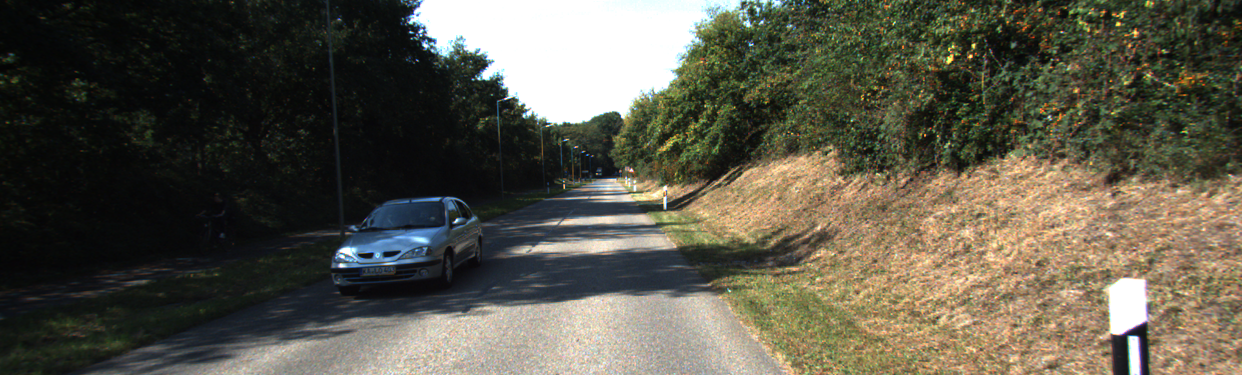
\includegraphics[width=0.99\linewidth]{Figures/56}
%                \caption{}
%        \end{subfigure}
%        \begin{subfigure}[t]{0.98\linewidth}
%                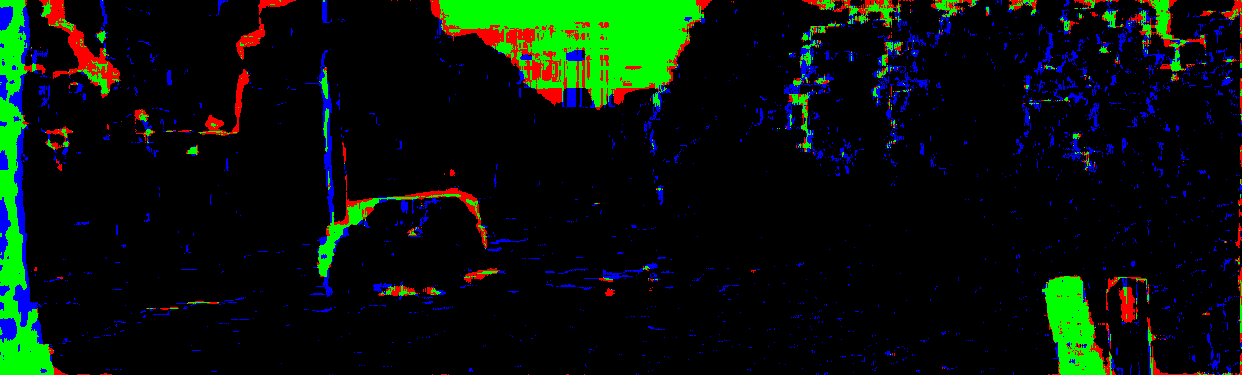
\includegraphics[width=0.99\linewidth]{Figures/Occ_56}
%                \caption{}
%        \end{subfigure}  
%        \caption{(a) \& (c) left image 003 \& 056 of KITTI 2015 training set, (b) \& (d) show pixels detected as ambiguous (threshold at $15$) with respect to LRC reference: true positive in green, over detection in red, and under-detection in blue.}
%\label{fig:occ} 
%\end{figure}

\begin{figure}[ht]
\centering        
        \begin{subfigure}[t]{0.98\linewidth}
                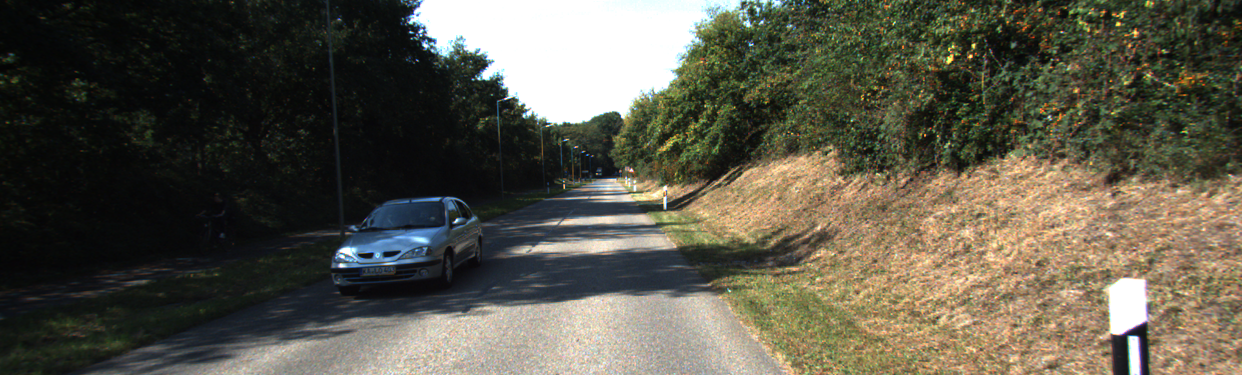
\includegraphics[width=0.99\linewidth]{Figures/56}
                \caption{}
        \end{subfigure}
        \begin{subfigure}[t]{0.98\linewidth}
                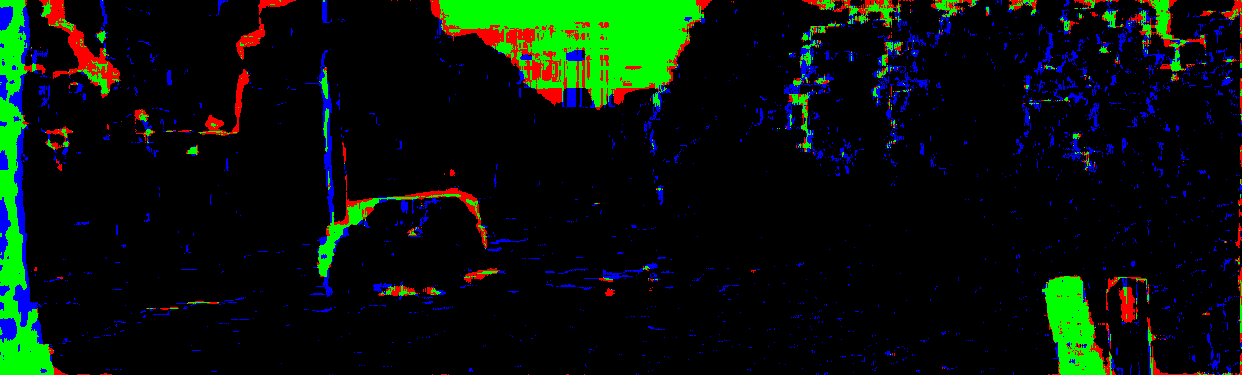
\includegraphics[width=0.99\linewidth]{Figures/Occ_56}
                \caption{}
        \end{subfigure}  
        \caption{(a) Left image 056 of KITTI 2015 training set, (b) shows pixels detected as ambiguous (threshold at $15$) with respect to LRC reference: true positive in green, over detection in red, and under-detection in blue.}
\label{fig:occ} 
\end{figure}

Fig.\ref{fig:occ} shows pixels in two scenes detected with a high ambiguity index with respect to LRC labels (``correct'' or non ``correct''): true positive in green, false positive in red, false negative in blue and true negative in black. Most occlusions are detected. Under-detection concerns thin objects or little discontinuities, and over-detection is mostly due to objects seen in right image but not in left image.

\subsection{Ambiguity Index as Data Uncertainty}

\begin{figure}[ht]
\centering
        \begin{subfigure}[t]{0.98\linewidth}
                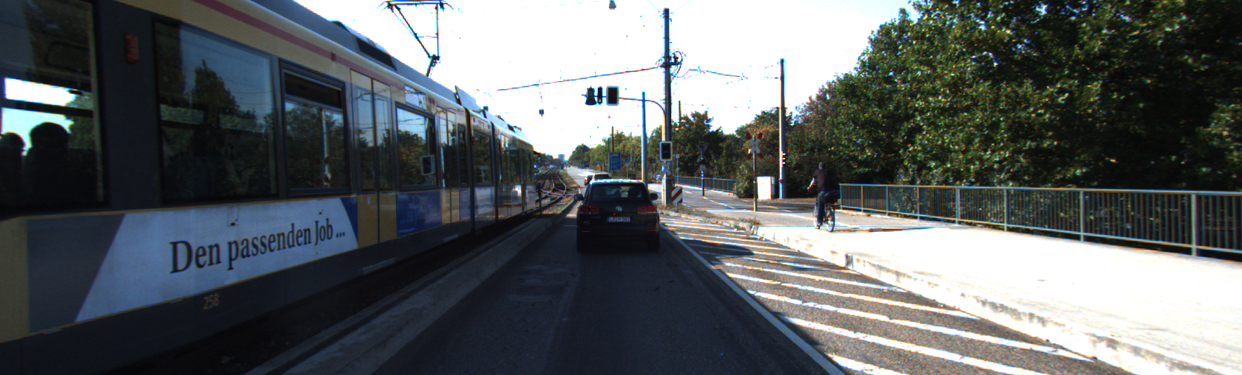
\includegraphics[width=0.99\linewidth]{Figures/144_10_il}
                \caption{Left image}
        \end{subfigure}
        \begin{subfigure}[t]{0.98\linewidth}
                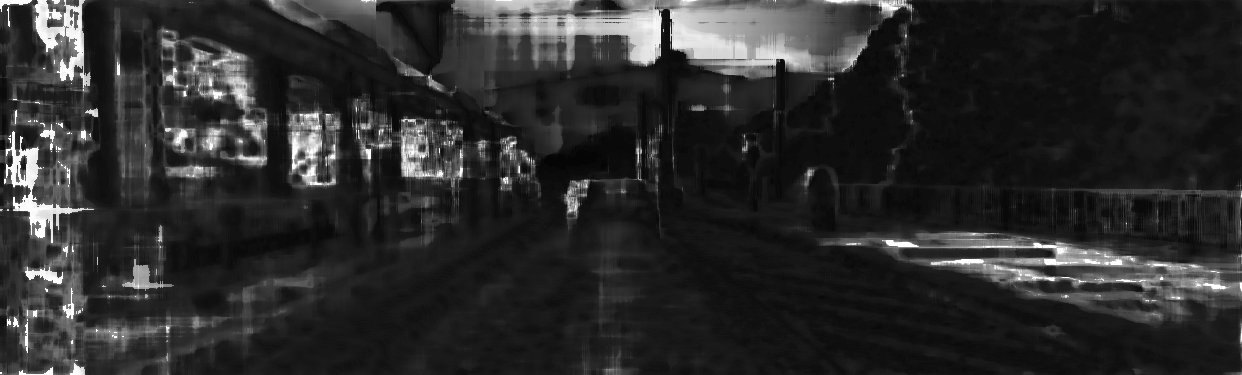
\includegraphics[width=0.99\linewidth]{Figures/144_10_ml2}
                \caption{Ambiguity index image}
        \end{subfigure}
        \begin{subfigure}[t]{0.98\linewidth}
                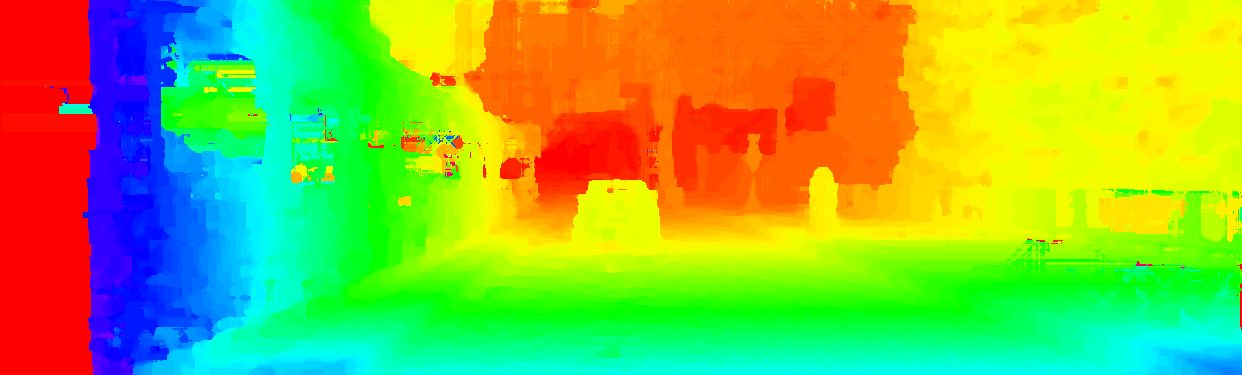
\includegraphics[width=0.99\linewidth]{Figures/144_10_df}
                \caption{Left disparity without index}
        \end{subfigure}        
        \begin{subfigure}[t]{0.98\linewidth}
                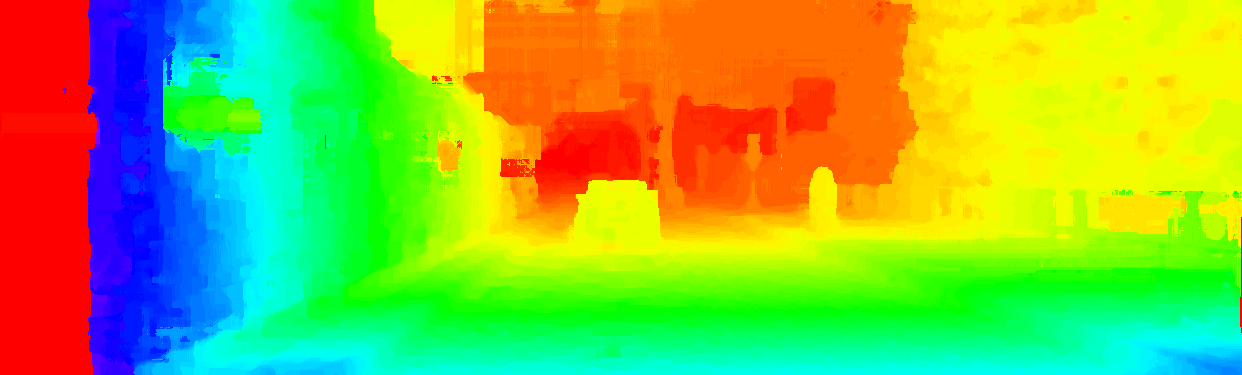
\includegraphics[width=0.99\linewidth]{Figures/144_10_df_}
                \caption{Left disparity with index weighting}
        \end{subfigure}        
        \caption{Results on image 144 of KITTI 2015 training set (a): Ambiguity index in (b), (c) disparity map without using the index, and (d) using the index. Higher index is whiter in (b).  Notice how reconstruction is improved on the tramway glasses between (c) and (d).}
        \label{fig:disp}
\end{figure}

We tested the second refinement method proposed in Sec.\ref{ss:in_proc} with $K=15$. Results are reported in the last line of Tab.~\ref{tab:KITTI}. What was observed with Refinement~1 method is confirmed with Refinement~2, with the difference that combination of LRC and Refinement~2 leads to even better improvements. On KITTI 2012, the obtained error rate is ranked 37, and for KITTI 2015, it is ranked between 10 to 15 (in January 2017) which is encouraging knowing that a better data cost (based on learning) than our simple census could be used.

A reconstruction result with and without the use of the index is shown Fig.\ref{fig:disp}, for illustration. Notice how the disparity map is improved on the tramway glasses. The ambiguity index detects reflections on the tramway glasses, saturated pixels in the sky and occlusion at the left of the car.

\section{Conclusion}
\label{sec:conclusion}

Our goal was to characterize the uncertainty of the disparity map estimated during stereo reconstruction process, a necessary but difficult task to perform. We proposed an ambiguity index designed to approximate the variances of every pixels of the estimated disparity map. This ambiguity index can only be computed when Dynamic Programming is used to solve the stereo reconstruction problem, as it is the case for the well known SGM optimization. In the experiments, it was shown that the proposed index has higher values where the data does not match with the model, for example in case of occlusion and in presence of specularities. This allows using the ambiguity index to improve the results by a post-processing, as shown experimentally with two proposed refinement methods on the KITTI 2012 and KITTI 2015 databases.  The proposed index can be also used for other kind of problems, provided the optimization is based on dynamic programming.

% References should be produced using the bibtex program from suitable
% BiBTeX files (here: strings, refs, manuals). The IEEEbib.bst bibliography
% style file from IEEE produces unsorted bibliography list.
% -------------------------------------------------------------------------
\bibliographystyle{IEEEbib}
\bibliography{refs}

\end{document}
